\documentclass[11pt]{beamer}
\usepackage[utf8]{inputenc}
\usepackage{graphicx, epsfig}
\usepackage{amsmath,mathrsfs,amsfonts,amssymb}
%\usepackage{subfig}
\usepackage{floatflt}
\usepackage{epic,ecltree}
\usepackage{mathtext}
\usepackage{fancybox}
\usepackage{fancyhdr}
\usepackage{multirow}
\usepackage{enumerate}
\usepackage{epstopdf}
\usepackage{multicol}
\usepackage{algorithm}
\usepackage[noend]{algorithmic}
\usepackage{tikz}
\usepackage{blindtext}
\usetheme{default}%{default}%{Singapore}%{Warsaw}%{Warsaw}%{Darmstadt}
\usecolortheme{default}
\setbeamerfont{title}{size=\Huge}
\setbeamertemplate{footline}[page number]{}


\makeatletter
\newcommand\HUGE{\@setfontsize\Huge{35}{40}}
\makeatother    

\setbeamerfont{title}{size=\HUGE}
\beamertemplatenavigationsymbolsempty

% latin bold lower
\newcommand{\ba}{\mathbf{a}} 
\newcommand{\bc}{\mathbf{c}} 
\newcommand{\be}{\mathbf{e}} 
\newcommand{\bh}{\mathbf{h}} 
\newcommand{\bp}{\mathbf{p}} 
\newcommand{\bt}{\mathbf{t}} 
\newcommand{\bs}{\mathbf{s}} 
\newcommand{\bu}{\mathbf{u}} 
\newcommand{\bv}{\mathbf{v}} 
\newcommand{\bw}{\mathbf{w}} 
\newcommand{\bx}{\mathbf{x}} 
\newcommand{\by}{\mathbf{y}} 
\newcommand{\bz}{\mathbf{z}} 

% latin bold upper
\newcommand{\bA}{\mathbf{A}} 
\newcommand{\bB}{\mathbf{B}} 
\newcommand{\bC}{\mathbf{C}} 
\newcommand{\bI}{\mathbf{I}} 
\newcommand{\bL}{\mathbf{L}} 
\newcommand{\bM}{\mathbf{M}} 
\newcommand{\bQ}{\mathbf{Q}} 
\newcommand{\bT}{\mathbf{T}} 
\newcommand{\bU}{\mathbf{U}} 
\newcommand{\bV}{\mathbf{V}} 
\newcommand{\bW}{\mathbf{W}} 
\newcommand{\bX}{\mathbf{X}} 
\newcommand{\bY}{\mathbf{Y}} 
\newcommand{\bZ}{\mathbf{Z}} 

% latin cal upper
\newcommand{\cG}{\mathcal{G}} 
\newcommand{\cL}{\mathcal{L}} 
\newcommand{\cN}{\mathcal{N}} 
\newcommand{\cS}{\mathcal{S}} 
\newcommand{\cT}{\mathcal{T}} 
\newcommand{\cW}{\mathcal{W}} 
\newcommand{\cX}{\mathcal{X}} 
\newcommand{\cZ}{\mathcal{Z}} 

% latin bb upper
\newcommand{\bbE}{\mathbb{E}} 
\newcommand{\bbI}{\mathbb{I}} 
\newcommand{\bbP}{\mathbb{P}} 
\newcommand{\bbR}{\mathbb{R}} 

% greek bold lower
\newcommand{\bepsilon}{\boldsymbol{\epsilon}} 
\newcommand{\btheta}{\boldsymbol{\theta}} 
\newcommand{\blambda}{\boldsymbol{\lambda}} 
\newcommand{\bpi}{\boldsymbol{\pi}} 
\newcommand{\bmu}{\boldsymbol{\mu}} 
\newcommand{\bsigma}{\boldsymbol{\sigma}} 
\newcommand{\bphi}{\boldsymbol{\phi}} 

% greek bold upper
\newcommand{\bSigma}{\boldsymbol{\Sigma}} 

\DeclareMathOperator*{\argmin}{arg\,min}
\DeclareMathOperator*{\argmax}{arg\,max}
\newcommand{\createdgmtitle}[1]{\title[\hbox to 56mm{Mathematical Forecasting Methods \hfill\insertframenumber\,/\,\inserttotalframenumber}]
	{\vspace{1.5\cm} \\ Mathematical Forecasting Methods \\ {\Huge Лекция #1}}
	\author{}
	\institute{
	МФТИ
	} 
	\date{Осень, 2023}
}

\newcommand\myfootnote[1]{%
  \tikz[remember picture,overlay]
  \draw (current page.south west) +(1in + \oddsidemargin,0.5em)
  node[anchor=south west,inner sep=0pt]{\parbox{\textwidth}{%
      \rlap{\rule{10em}{0.4pt}}\raggedright\scriptsize \textit{#1}}};}

\newcommand\myfootnotewithlink[2]{%
  \tikz[remember picture,overlay]
  \draw (current page.south west) +(1in + \oddsidemargin,0.5em)
  node[anchor=south west,inner sep=0pt]{\parbox{\textwidth}{%
      \rlap{\rule{10em}{0.4pt}}\raggedright\scriptsize\href{#1}{\textit{#2}}}};}
\createdgmtitle{4}
\usepackage{tikz}
\usepackage{amsmath}
\usepackage[english,russian]{babel}
\usepackage[labelformat=empty]{caption}

\usepackage{graphicx,animate}
\usepackage{animate}
\usepackage{caption}
\usepackage{subcaption}

\usetikzlibrary{arrows,shapes,positioning,shadows,trees}
\newcommand*{\defeq}{\stackrel{\text{def}}{=}}

%--------------------------------------------------------------------------------
\begin{document}
%--------------------------------------------------------------------------------
\begin{frame}[plain]
%\thispagestyle{empty}
\titlepage
\end{frame}
%=======
\begin{frame}{Forecasting Methods/Models zoo}
    \begin{figure}
        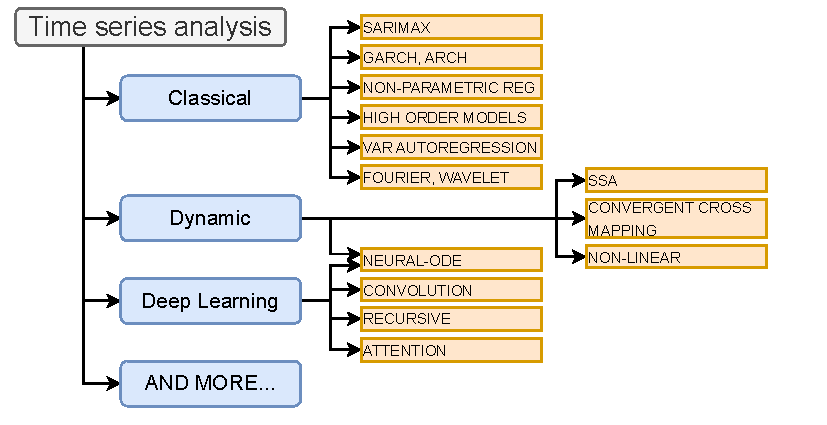
\includegraphics[width=1.1\linewidth, left]{./figs/init_diagram.pdf}
    \end{figure}
\end{frame}
%======
\begin{frame}{Элементы теории динамических систем}

Теория динамических систем изучает процессы, которые развиваются во времени. 
Описание этих процессов дается в терминах разностных или дифференциальных
уравнений или последовательности преобразований.
\newline{}
\textbf{Динамическая система} --- это система, которая эволюционирует (меняется) со временем согласно некоему закону.
\begin{figure}
    \centering
    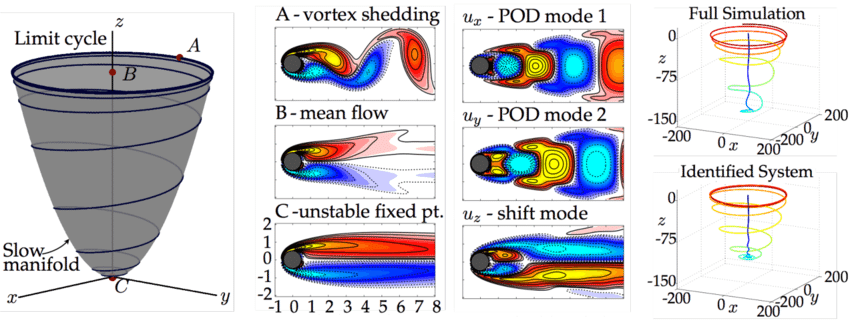
\includegraphics[width=0.8\textwidth]{lecture_4/figs/example-1.png}
\end{figure}

\end{frame}
%=======
\begin{frame}{Элементы теории динамических систем}

Теория динамических систем изучает процессы, которые развиваются во времени. 
Описание этих процессов дается в терминах разностных или дифференциальных
уравнений или последовательности преобразований.
\newline{}
\textbf{Динамическая система} --- это система, которая эволюционирует (меняется) со временем согласно некоему закону.
\begin{figure}
    \centering
    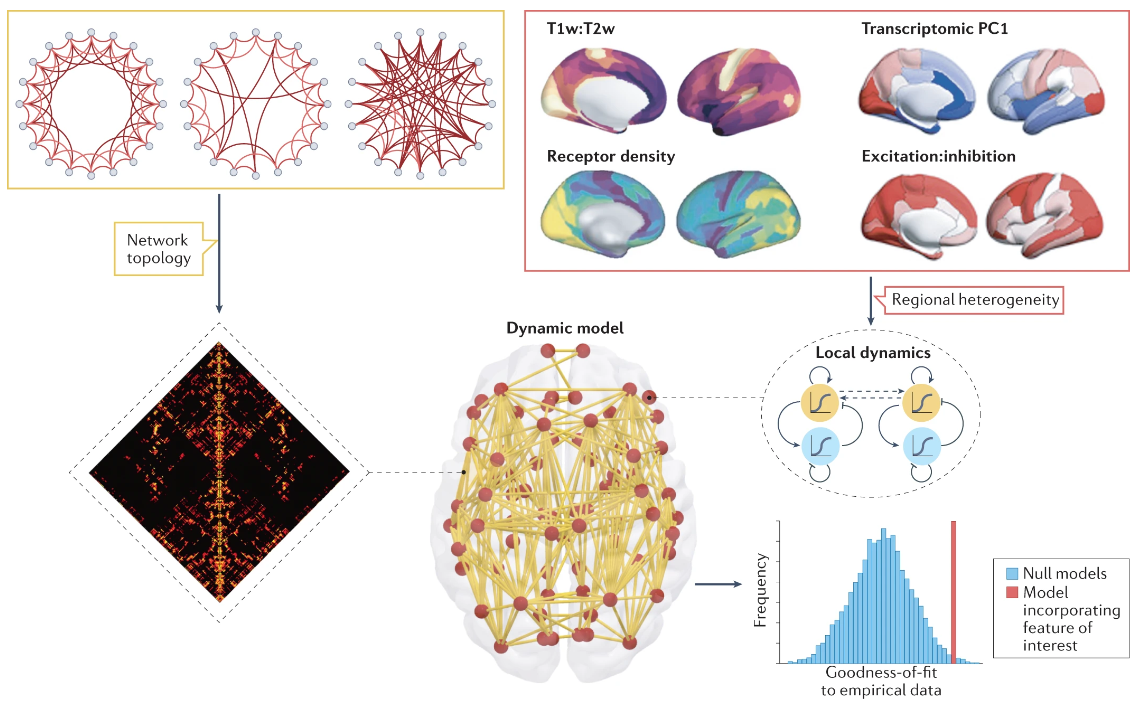
\includegraphics[width=0.65\textwidth]{lecture_4/figs/example-2.png}
\end{figure}

\end{frame}
%=======
\begin{frame}{Динамическая система}
Определение динамической системы включает в себя три компоненты:
\begin{itemize}
    \item фазовое пространство (также называемое пространством состояний)
    \item время
    \item закон эволюции
\end{itemize}

\begin{figure}
    \centering
    \animategraphics[autoplay,loop,width=1\textwidth]{10}{lecture_4/figs/gif_1/frame-}{0}{38}
\end{figure}

\end{frame}
%=======
\begin{frame}{Динамическая система}
\textbf{Фазовое пространство} --- это множество, элементы которого (называемые “точками”) представляют возможные состояния системы* в любой момент времени.

\vspace{0.5cm}
\textbf{Время} может быть либо дискретным, либо непрерывным.

\vspace{0.5cm}
\textbf{Закон эволюции} --- это правило, которое позволяет, если известно состояние системы в какой-то момент времени, определить состояние системы в любой другой момент времени. Предполагается, что процесс детерминирован в прошлом и в будущем. \\
\vspace{0.5cm}
*Одна и та же динамическая система может описываться с помощью разных фазовых пространств и разных векторов состояний -- предпочтительным, как правило, является наиболее низкоразмерное описание.

\end{frame}
%=======
\begin{frame}{Теория динамических систем}
Модель динамической системы -- функция, описывающая динамику системы в терминах дифференциального уравнения:
$$ \frac{\text{d}\mathbf{x}}{\text{d}t} = \mathbf{f}\Big(\mathbf{x}(t), t, \mathbf{u}(t), \beta \Big) + n, $$
где $\mathbf{x}$ -- состояние системы, $t$ -- время, $\mathbf{u}$ -- управление, $\beta$ -- параметры, $n$ -- шум. \\
Альтернатива -- рекуррентное соотношение $\mathbf{x}_{k+1} = \mathbf{F}
(\mathbf{x}_k)$.

Проблемы:
\begin{enumerate}
    \item Функция $\mathbf{f}$ зачастую неизвестна.
    \item Функция $\mathbf{f}$ зачастую нелинейна.
    \item Как правило, $\mathbf{x} \in \mathbb{R}^n$, а $n$ может быть очень большим.
    \item Распределение шума неизвестно.
    \item Что должно выступать в качестве состояния $\mathbf{x}$? (проблема выбора "координат")
\end{enumerate}
\end{frame}
%=======
\begin{frame}{Зачем моделировать динамические системы?}

\begin{itemize}
\item \textbf{Предсказание}: мы хотим предвидеть поведение системы в будущем (метеорология, климатология и т.д.)
\item \textbf{Оптимизация/дизайн}: введение параметров в модель динамической системы позволяет нам изучать её поведение в зависимости от параметров и находить их оптимальные значения.
\item \textbf{Управление}: введение управления в описание системы позволяет нам изучать отклик системы на внешнее контролируемое воздействие в реальном времени и моделировать управляемые системы.
\item \textbf{Интерпретация и физический смысл}: анализ поведения, параметров и траекторий моделируемой динамической системы позволяет лучше понять её физическую природу. 
\end{itemize}
\end{frame}
%=======
\begin{frame}{Зачем моделировать динамические системы?}
\begin{figure}
    \centering
    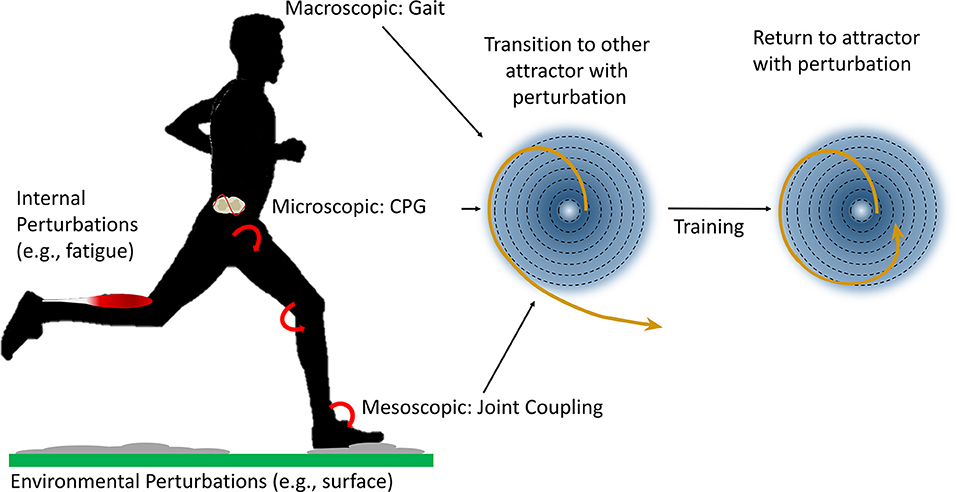
\includegraphics[width=\textwidth]{lecture_4/figs/DS-1.jpg}
\end{figure}

\end{frame}
%=======
\begin{frame}{Вектор задержек (Delay embedding)}
Временным рядом $\{x_i\}_1^N $ называется массив из N чисел
\begin{itemize}
    \item представляющих собой значения некоторой измеренной (наблюдаемой) динамической переменной $\textbf{x}(t)$,
    \item с некоторым постоянным шагом $\Delta t$ по времени.
\end{itemize} 
 Зачастую временной ряд удобно представить в виде \textit{фазовых траекторий} 
-- вместо переменных, входящих в систему, использовать векторы задержек: $\mathbf{z}_i = [x_i, x_{i-1}, ..., x_{i-m+1}]$. Один такой вектор является элементом $m$-мерного фазового пространства $\mathbb{R}^m$.

\begin{figure}
    \centering
    \animategraphics[autoplay,loop,width=0.8\textwidth]{10}{lecture_4/figs/gif_2/frame-}{0}{39}
\end{figure}

\end{frame}
%=======
\begin{frame}{Элементы теории Такенса}
\begin{itemize}
    \item Пусть задана динамическая система $f(\mathbf{x})$ с фазовым пространством $\mathbb{R}^M$.
    \item Величины, образующие временной ряд, являются значениями некоторой функции $h$ состояния $\mathbf{x}(t)$ этой динамической системы на многообразии $W^d \subset \mathbb{R}^M$: $h:W^d \rightarrow \mathbb{R}, \quad x_i = h(\mathbf{x}(t_i)) = h(f(\mathbf{x}_0,t_i))$. 
    \item При фиксированном шаге во времени $\Delta t$: $\mathbf{x}(t) = f(\mathbf{x}_0,t_i + i \cdot \Delta t)$.
\end{itemize}
Поэтому для компонент векторов задержки выполняется:

$$ x_i = h(\mathbf{x}(t_i)) = h(f(\mathbf{x}_0,t_i)) $$
$$ x_{i+1} = h(\mathbf{x}(t_{i+1})) = h(f(\mathbf{x}_0,t_i + \Delta t)) $$
$$ \dots $$
$$ x_{i+m-1} = h(\mathbf{x}(t_{i + m - 1})) = h(f(\mathbf{x}_0,t_i + (m-1)\cdot \Delta t) $$


\end{frame}
%=======
\begin{frame}{Элементы теории Такенса}

Поскольку все компоненты вектора $\mathbf{z}_i = [x_i, x_{i - 1}, ..., x_{i+m - 1}]$ можно связать с одним и тем же измерением состояния динамической системы $x_i =  h(f(\mathbf{x}_0,t_i))$, то существует векторная функция $\Lambda$, отображающая $x_i$ в векторы $m$-мерного пространства $\mathbb{R}^m$:
$$
\mathbf{z}_i = \Lambda(x_i),  \quad \mathbf{z}_i \in \mathbb{R}^m.
$$
Приведенные рассуждения и составляют основное содержание теоремы
Такенса, утверждающей, что при $m \geq 2d + 1$ свойством
отображения $\Lambda$ является вложение $W^d$ в $\mathbb{R}^m$.

\end{frame}
%=======
\begin{frame}{Элементы теории Такенса}
\begin{figure}
    \centering
    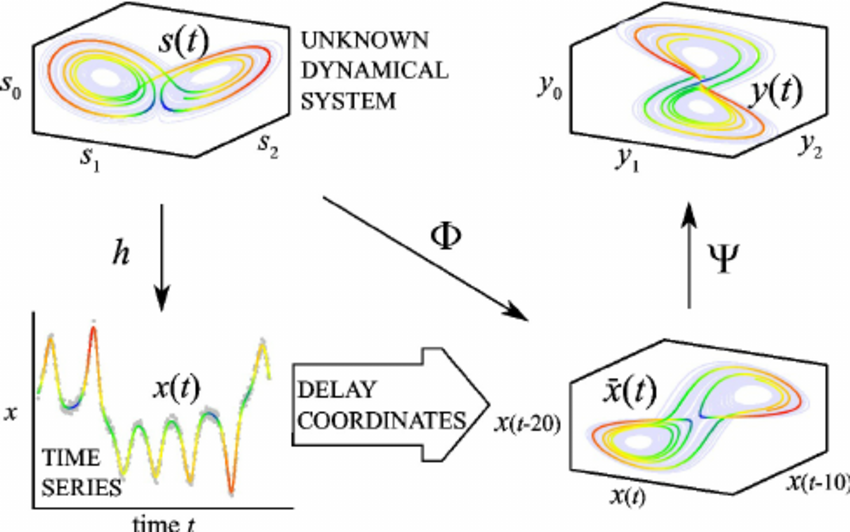
\includegraphics[width=\textwidth]{lecture_4/figs/CCM-1.png}
\end{figure}
\end{frame}
%=======
\begin{frame}{Выводы из теоремы Такенса}
\begin{itemize}
    \item  В соответствии с теорией Такенса приемлемое описание фазового пространства динамической
системы можно получить, если взять вместо реальных переменных системы  $m$–мерные векторы задержек, составленные из значений ряда в последовательные моменты времени.
    \item При выполнении условия $m \geq 2d + 1$, где $d$ — размерность вложения, возможно реконструировать пространство состояний системы.
    \item При условии стационарности временного ряда на базе этой реконструкции строится прогноз его дальнейшей динамики.
\end{itemize}
\end{frame}
%=======
\begin{frame}{Методы поиска $m$}
\begin{itemize}
    \item На сегодняшний день наиболее часто используемым алгоритмом для оценки величины $m$ является алгоритм Грассбергера–Прокаччиа (метод оценки, основанный на расстояниях в фазовых пространствах).
    \item Имеются также и другие методы, среди которых наиболее приемлемый — это т.н. функциональный метод.
    \item Зачастую из-за сложности методов величина $m$ определяется эмпирически.
    \item \textbf{Главный критерий} --- выбор такого $m$, начиная с которого \textbf{прекращается качественное изменение прогноза}.
\end{itemize}

\end{frame}
%=======
\begin{frame}{Проблемы выбора $\tau$}
\begin{itemize}
    \item Малые значения могу затеряться в шумовой компоненте сигнала
    \item Большие значения --- малоинформативны из-за слабой связи между измерениями
    \item При плохо подобранном $m$ появляется проблема оценки близости в фазовом пространстве
\end{itemize}

\begin{figure}
 \begin{subfigure}[b]{0.24\textwidth}
    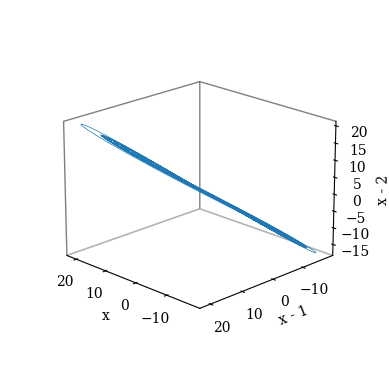
\includegraphics[width=\linewidth]{lecture_4/figs/tde_lorenz_tau_1.png}
    \caption{$\tau=1$}
  \end{subfigure}
  \begin{subfigure}[b]{0.24\textwidth}
    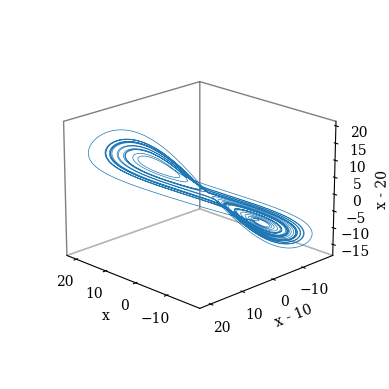
\includegraphics[width=\linewidth]{lecture_4/figs/tde_lorenz_tau_10.png}
    \caption{$\tau=10$}
  \end{subfigure}
  \begin{subfigure}[b]{0.24\textwidth}
    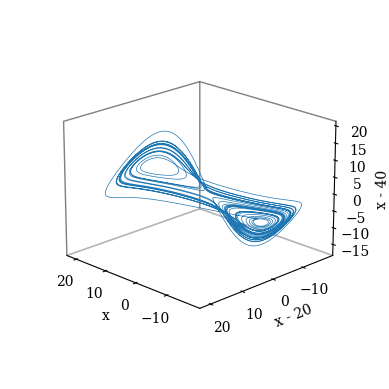
\includegraphics[width=\linewidth]{lecture_4/figs/tde_lorenz_tau_20.png}
    \caption{$\tau=20$}
  \end{subfigure}
  \begin{subfigure}[b]{0.24\textwidth}
    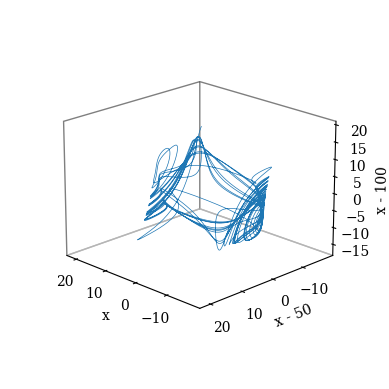
\includegraphics[width=\linewidth]{lecture_4/figs/tde_lorenz_tau_50.png}
    \caption{$\tau=50$}
  \end{subfigure}
\end{figure}

\end{frame}
%=======
\begin{frame}{Проблемы выбора $\tau$}
\begin{itemize}
    \item Малые значения могу затеряться в шумовой компоненте сигнала
    \item Большие значения --- малоинформативны из-за слабой связи между измерениями
    \item При плохо подобранном $m$ появляется проблема оценки близости в фазовом пространстве
\end{itemize}

\begin{figure}
    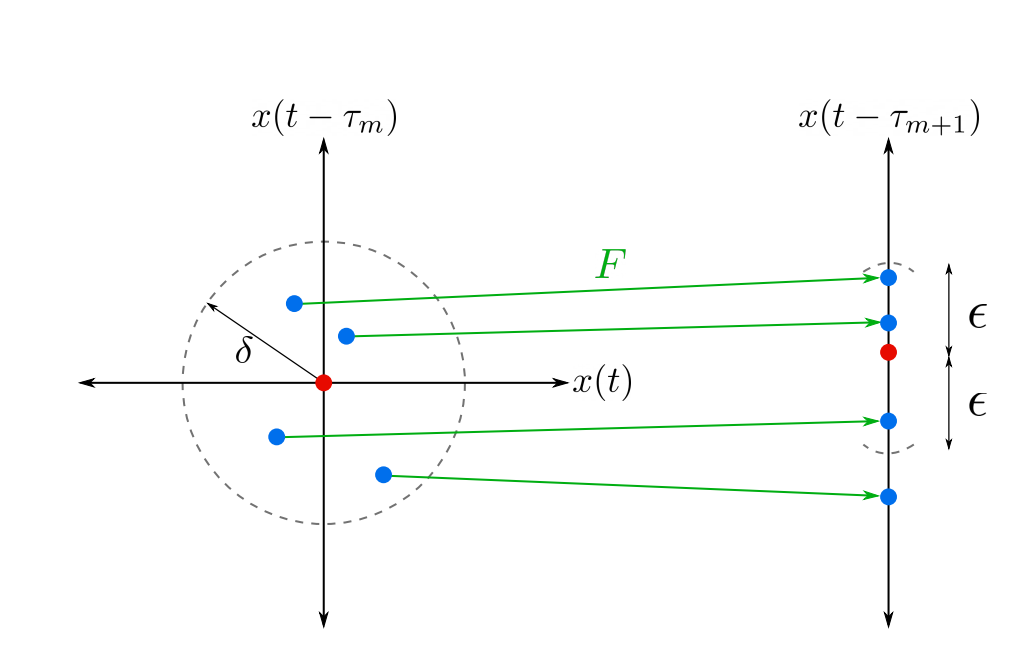
\includegraphics[width=0.7\linewidth]{lecture_4/figs/nn_problem.png}
\end{figure}

\end{frame}
%=======
\begin{frame}{Проблемы выбора $\tau$}
\begin{itemize}
    \item Часто используемая эвристика --- $\tau$ как четверть наиболее доминирующего периода в сигнале.
    \item  Эта эвристика основана на задача вложения синусоиды в 2D $x(t) = \test{sin}(\omega t)$.
    \item  При $ \tau = \frac{2\pi}{4\omega}$ метод восстанавливает круговую траекторию. Другие значения приводят к эллиптическим траекториям.
    \item Эта эвристика не может быть  применено к хаотическим системам, где сигналы апериодические.
\end{itemize}

\begin{figure}
    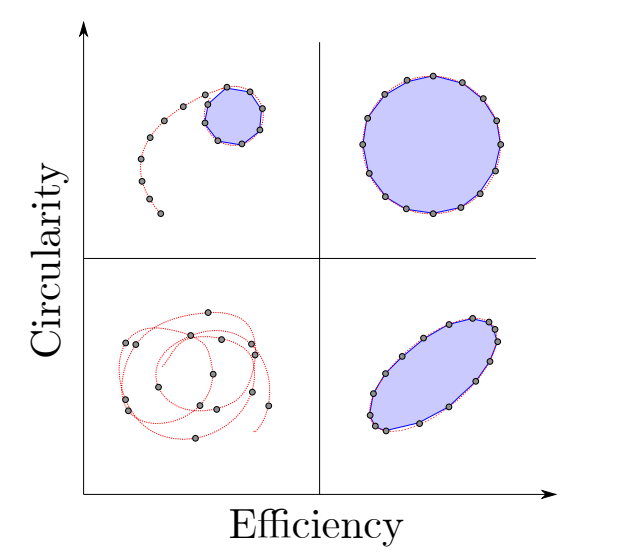
\includegraphics[width=0.45\linewidth]{lecture_4/figs/2d_case.png}
\end{figure}

\end{frame}
%=======
\begin{frame}{Проблемы выбора $\tau$}
\begin{itemize}
    \item Подход на основе моделей снижения размерности
    \item В подходе используются большие $m$ и малые $\tau$ для снижения размерности до некоего малого значения
    \item Часто используется метод главных компонент
\end{itemize}

\begin{figure}
    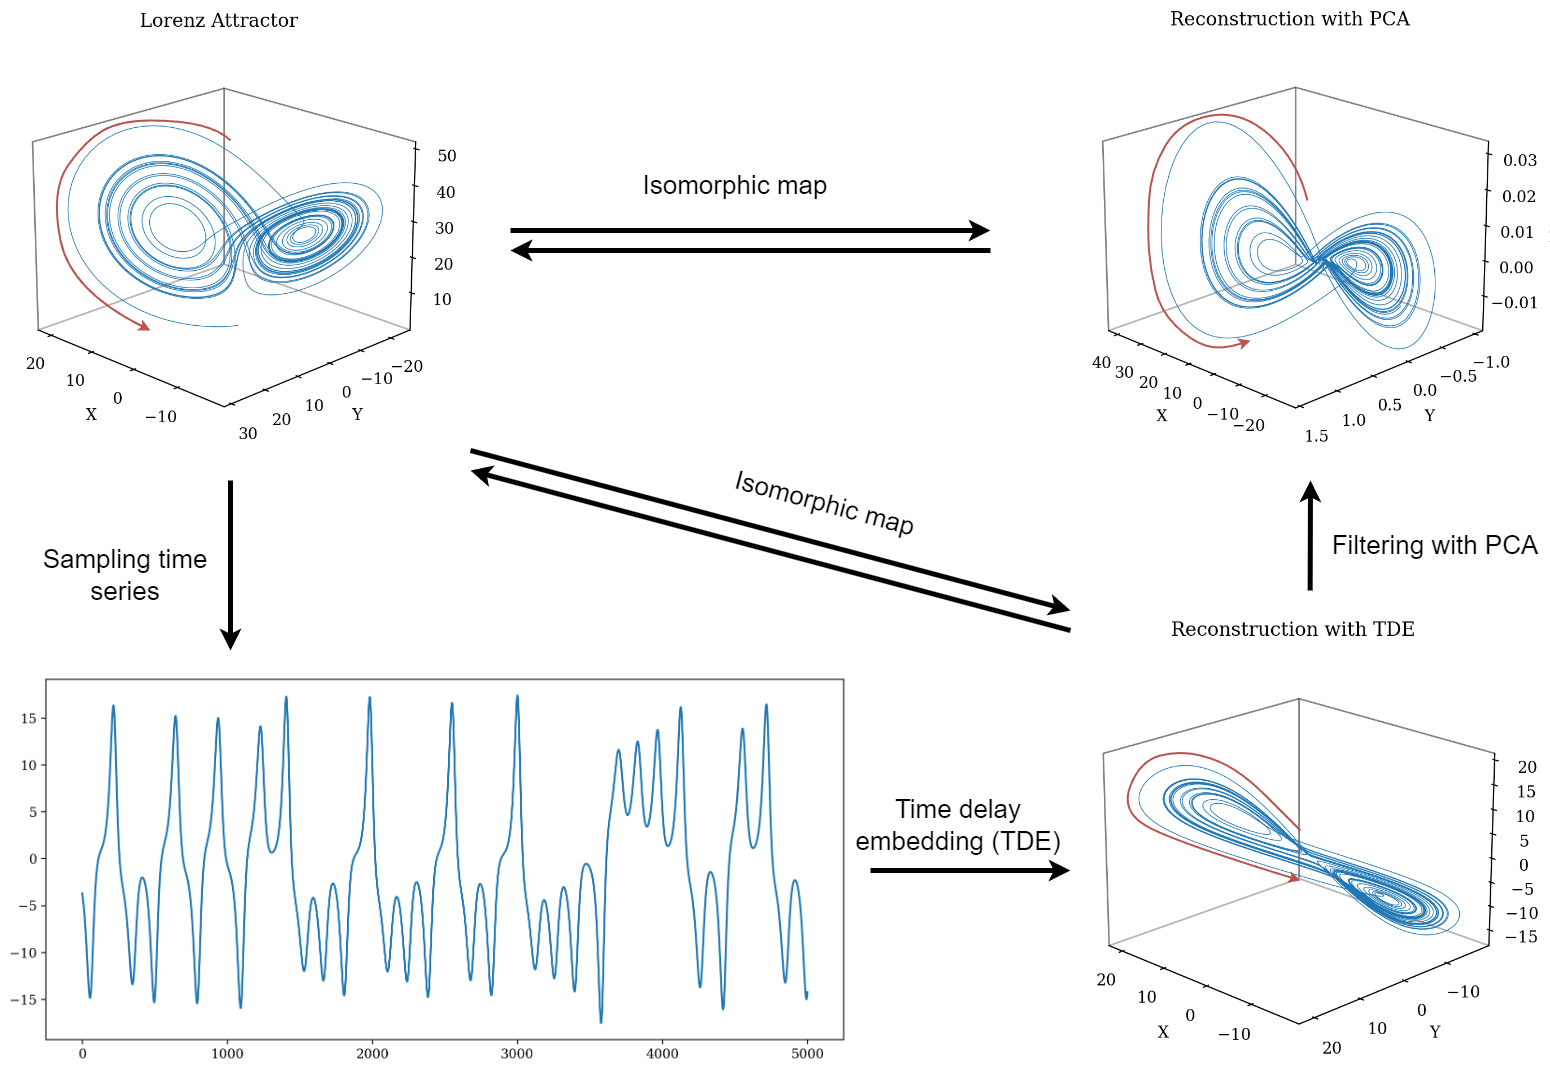
\includegraphics[width=0.7\linewidth]{lecture_4/figs/init_schema_2.png}
\end{figure}

\end{frame}
%=======


\begin{frame}{Идея алгоритма Convergent Cross Mapping}

\begin{itemize}
    \item Пусть имеется пара динамических систем $X$ и $Y$, истинное поведение которых описывается многообразиями $W_x$ и $W_y$ в соответствующих фазовых пространствах.
Об этих многообразиях мы можем судить лишь по их проекциям $M_x$ и $M_y$ на измеренные значения временных рядов $\{x_t\}_{t=1}^T$ и $\{y_t\}_{t=1}^T$, соответствующих данным системам.
    \item (\textbf{Cross Mapping}) По фазовой траектории одной из систем $M_x$ можно предсказывать значения второй системы $y_t \simeq \hat{y}_t|M_x$. Аналогично, можно строить и предсказания $\hat{x}_t|M_y$ . По точности данных предсказаний можно судить о наличии причинно-следственной связи между системами.
    \item (\textbf{Convergence}) При этом, если такая связь существует, то качество предсказания должно расти при увеличении рассматриваемого временного отрезка $T$.
    
\end{itemize}

\end{frame}
%=======
\begin{frame}{Иллюстрация Cross Convergent Mapping}
\begin{figure}
    \centering
    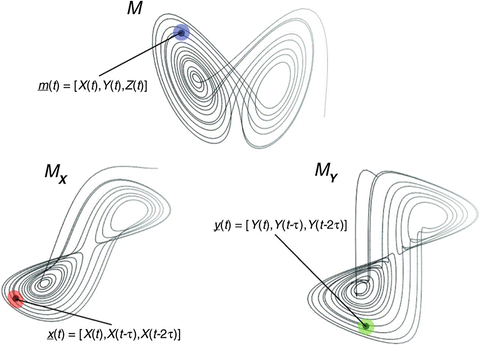
\includegraphics[width=\textwidth]{lecture_4/figs/CCM.png}
\end{figure}
\end{frame}
%=======

\begin{frame}{Алгоритм Convergent Cross Mapping}

\begin{enumerate}
    \item Пусть имеются 2 временных ряда $\{x_1, x_2,...,x_T\}$ и $\{y_1, y_2,...,y_T\}$ длины $T$.
    \item Для ряда $\{x_t\}_{t=1}^T$ формируем векторы предыстории размерности $E$ с шагом по времени $\tau$:
    $$ \mathbf{x}_t = \begin{pmatrix}
        x_t, & x_{t - \tau}, & x_{t - 2\tau}, & \dots, & x_{t - (E-1)\tau}
    \end{pmatrix}$$
    \item В пространстве $\mathbb{R}^E$ (\textit{фазовом пространстве}) такие векторы предыстории образуют\textit{фазовую траекторию} системы -- множество $M_x = \{\mathbf{x}_t \ | \ t = 1 + (E - 1)\tau, ..., T \}$.
    \item[4.] Пусть требуется построить предсказание для значения $y_t$. Для этого сначала найдем $E + 1$ векторов из $M_x$, ближайших к $\mathbf{x}_t$ (в терминах, например, стандартной метрики $d$ в $\mathbb{R}^n$). Пусть им соответствуют временные индексы $t_1, ..., t_{E+1}$, отсортированные в порядке от ближайшей точки до наиболее удалённой.
    $$ d_i = d(\mathbf{x}_t, \mathbf{x}_{t_i}), \quad d_1 < d_2 < ... < d_{E + 1}$$
\end{enumerate}

\end{frame}
%=======

\begin{frame}{Алгоритм Convergent Cross Mapping}

\begin{enumerate}

    \item[5.] Тогда оценка значения $y_t$ строится следующим образом в виде взвешенной суммы значений ряда в моменты времени $t_1, ..., t_{E+1}$:
    $$ \hat{y}_t|M_x = \sum_{i=1}^{E+1} \omega_i y(t_i)$$
    $$ \omega_i = \frac{u_i}{\displaystyle \sum_{j=1}^{E + 1}u_j}, \quad \quad u_i = e^{\displaystyle - \frac{d_i}{d_1}}, \quad \quad i = 1, ..., E+1$$
    \item[6.] Для того, чтобы посудить о существовании зависимости между рядами $\{x_t\}_{t=1}^T$ и $\{у_t\}_{t=1}^T$, рассчитаем теперь коэффициент корреляции Пирсона:
    $$ C_{yx} = \Bigg[\rho \Big( y, \hat{y}|M_x \Big) \Bigg]^2$$

\end{enumerate}

\end{frame}
%=======

\begin{frame}{Резюме}
\begin{itemize}
    \item Временной ряд -- это характеристика состояния динамической системы (набор значений некоторой функции состояния).
    \item Математические основы динамических систем позволяют осуществлять анализ временных рядов.
    \item Теорема Такенса позволяет использовать вектора задержек для восстановления внутренней структуры динамической системы.
    \item В частности, выводы теоремы Такенса используются в CCM. Алгоритм CCM является аналогом статистического теста и оценивает причинно-следственную связь двух временных рядов.
\end{itemize}
\end{frame}
\end{document} 